        %%******************************************%%
        %%                                          %%
        %%        Modello di tesi di laurea         %%
        %%            di Andrea Giraldin            %%
        %%                                          %%
        %%             2 novembre 2012              %%
        %%                                          %%
        %%******************************************%%

\begin{document}
    \frontmatter
    \begin{titlepage}
    % University info at the top
    \begin{center}
        \begin{LARGE}
            \textbf{\myUni}\\
        \end{LARGE}

        \vspace{10pt}

        \begin{Large}
            \textsc{\myDepartment}\\
        \end{Large}

        \vspace{10pt}

        \begin{large}
            \textsc{\myFaculty}\\
        \end{large}
    \end{center}

    % Center the title vertically in the remaining space
    \vspace*{\fill}
    \begin{center}
        \begin{LARGE}
            \textbf{\myTitle}\\
        \end{LARGE}

        \vspace{20pt}

        \begin{large}
            \textsl{\myDegree}\\
        \end{large}
    \end{center}

    % Other data at the bottom
    \vfill
    \begin{center}
        \begin{large}
            \begin{flushleft}
                \textit{Relatore}\\
                \vspace{5pt}
                \profTitle\ \myProf
            \end{flushleft}

            \begin{flushright}
                \textit{Laureando}\\
                \vspace{5pt}
                \myName \\
                \vspace{5pt}
                \textit{Matricola} \myID
            \end{flushright}
        \end{large}

        \vspace{40pt}

        \line(1, 0){338} \\
        \begin{normalsize}
            \textsc{Anno Accademico \myAA}
        \end{normalsize}
    \end{center}
\end{titlepage}

    % \clearpage
\phantomsection
\thispagestyle{empty}

\hfill
\vfill

\noindent\myName: \textit{\myTitle,}
\myDegree,
\textcopyright\ \myTime.

    % \cleardoublepage
\phantomsection
\thispagestyle{empty}
\pdfbookmark{Dedica}{Dedica}

\vspace*{3cm}

\begin{center}
    Lorem ipsum dolor sit amet, consectetuer adipiscing elit. \\ \medskip
    --- Oscar Wilde
\end{center}

\medskip

\begin{center}
    Dedicato a ...
\end{center}

    \cleardoublepage
\phantomsection
\pdfbookmark{Sommario}{Sommario}
\begingroup
\let\clearpage\relax
\let\cleardoublepage\relax
\let\cleardoublepage\relax

\chapter*{Sommario}

Il presente documento riporta le attività svolte durante il periodo di stage della durata complessiva di circa 300 ore, svolto dal laureando Eghosa Matteo Igbinedion Osamwonyi presso Halue S.r.l. Società Benefit.  
Lo stage aveva come obiettivo principale la progettazione e lo sviluppo di un prototipo di interfaccia conversazionale per il sito e-commerce di un brand di skincare con integrazione a favore dell'esperienza utente, basata su un'architettura agentica. Il sistema proposto integra Large Language Models (LLM), Retrieval-Augmented Generation (RAG) e agenti software (agent MCP), e prevede connettori verso il backend Shopify per reperire dati ed eseguire azioni automatizzate.  
Le attività svolte comprendono l'analisi del dominio e dei requisiti, la progettazione architetturale modulare (microservizi), lo sviluppo del proof-of-concept operativo, l'integrazione del modulo RAG e i test end-to-end. Sono inoltre previste soluzioni per il fallback in caso di incertezza del modello e opzioni per la gestione dinamica dei contenuti.  
I prodotti attesi sono: (1) un prototipo funzionante del sistema conversazionale; (2) la relazione tecnica che documenta analisi, progettazione e risultati.

\endgroup

\vfill

    %\cleardoublepage
\phantomsection
\pdfbookmark{Ringraziamenti}{ringraziamenti}

\begin{flushright}{
    \slshape
    ``Life is really simple, but we insist on making it complicated''} \\
    \medskip
    --- Confucius
\end{flushright}


\bigskip

\begingroup
\let\clearpage\relax
\let\cleardoublepage\relax
\let\cleardoublepage\relax

\chapter*{Ringraziamenti}

\noindent \textit{Innanzitutto, vorrei esprimere la mia gratitudine al Prof. \myProf, relatore della mia tesi, per l'aiuto e il sostegno fornitomi durante la stesura del lavoro.}\\

\noindent \textit{Desidero ringraziare con affetto i miei genitori per il sostegno, il grande aiuto e per essermi stati vicini in ogni momento durante gli anni di studio.}\\

\noindent \textit{Ho desiderio di ringraziare poi i miei amici per tutti i bellissimi anni passati insieme e le mille avventure vissute.}\\
\bigskip

\noindent\textit{\myLocation, \myTime}
\hfill \myName

\endgroup

    \cleardoublepage
\pdfbookmark{\contentsname}{tableofcontents}
\setcounter{tocdepth}{2}
\tableofcontents
%\markboth{\contentsname}{\contentsname}
\clearpage

\begingroup
    \let\clearpage\relax
    \let\cleardoublepage\relax
    \let\cleardoublepage\relax

    % Figures list
    \phantomsection
    \pdfbookmark{\listfigurename}{lof}
    \listoffigures

    \vspace*{8ex}

    % Tables list
    \phantomsection
    \pdfbookmark{\listtablename}{lot}
    \listoftables

    \vspace*{8ex}
\endgroup

\cleardoublepage

    \cleardoublepage

    \mainmatter
    %\input{chapters/introduzione}
    \chapter{Azienda}
\label{cap:azienda}

%\intro{Introduzione al capitolo sull'azienda}\\

\section{Descrizione generale}

Le principali fonti di informazione relative all'azienda ospitante derivano dalla consultazione del \emph{sito web} aziendale, effettuata durante la fase di scelta dello stage, 
e dalle interazioni con il tutor aziendale e i membri del team nelle prime fasi conoscitive. Poiché la mia postazione era nella stessa stanza del team nei giorni di presenza in azienda, 
ho inoltre raccolto informazioni di tipo informale osservando il lavoro quotidiano e ascoltando le conversazioni del gruppo. Le informazioni non sono state tutte disponibili prima dell'inizio del progetto, 
ma si sono accumulate gradualmente durante l'intero periodo di stage.

Halue S.r.l. è una società benefit di consulenza tecnica orientata all'adozione di soluzioni basate sull'intelligenza artificiale e alla fornitura di servizi 
sia \emph{B2C} (business-to-consumer) sia \emph{B2B} (business-to-business). 
Le attività dell'azienda si articolano in diversi servizi, tra cui: progettazione e gestione di soluzioni per l'\emph{e-commerce} (commercio elettronico), 
implementazione di sistemi di gestione delle relazioni con i clienti (\emph{CRM}, Customer Relationship Management), 
servizi legati all'IA (ad es. sviluppo di agenti intelligenti) e percorsi di formazione rivolti ai clienti.

\medskip
\noindent\textbf{Contesto organizzativo}

Le informazioni relative al contesto organizzativo derivano sia dalle discussioni con il tutor aziendale sull'andamento del progetto, 
sia dalle conversazioni con altri membri del team. L'organizzazione concilia modalità di lavoro ibride e in \emph{full remote}. 
Il team tiene \emph{stand-up meeting} quotidiani per allinearsi sul lavoro svolto nella giornata precedente e sugli obiettivi della giornata corrente; 
periodicamente vengono organizzati incontri informali per mantenere buoni rapporti fra i membri e rinsaldare i valori aziendali.

La comunicazione interna si sviluppa su più livelli, con strumenti scelti in funzione delle esigenze organizzative:

\begin{itemize}
\item richieste di aiuto di carattere informale vengono spesso rivolte verbalmente; richieste più dettagliate o tecniche vengono inserite nello strumento di gestione dei progetti, dove ogni membro può \emph{postare} dubbi o proposte all'interno del proprio ramo di lavoro;
\item richieste di \emph{meeting} o chiarimenti che richiedono l'accordo su un orario sono gestite tramite la piattaforma di messaggistica condivisa dal team;
\item infine, le comunicazioni di natura amministrativa o burocratica vengono inviate tramite Gmail.
\end{itemize}

\medskip
\noindent\textbf{Contesto produttivo}

Le informazioni sul contesto produttivo provengono dalle interazioni con il tutor e dai colloqui con i colleghi. 
Dal punto di vista produttivo, l'azienda privilegia il rapido ingresso delle soluzioni nel mercato, adottando architetture che riducano gli ostacoli al 
\emph{deployment} (messa in distribuzione del software in ambiente operativo). Ho riscontrato l'uso dell'approccio \emph{Agile} (metodologie iterative e incrementali per adattarsi rapidamente ai cambiamenti dei requisiti) 
con gestione tramite \emph{backlog} (elenco prioritizzato di attività) e strumenti di tracciamento. La comunicazione interna è adattata alle necessità operative.

\begin{figure}[htbp]
    \centering
    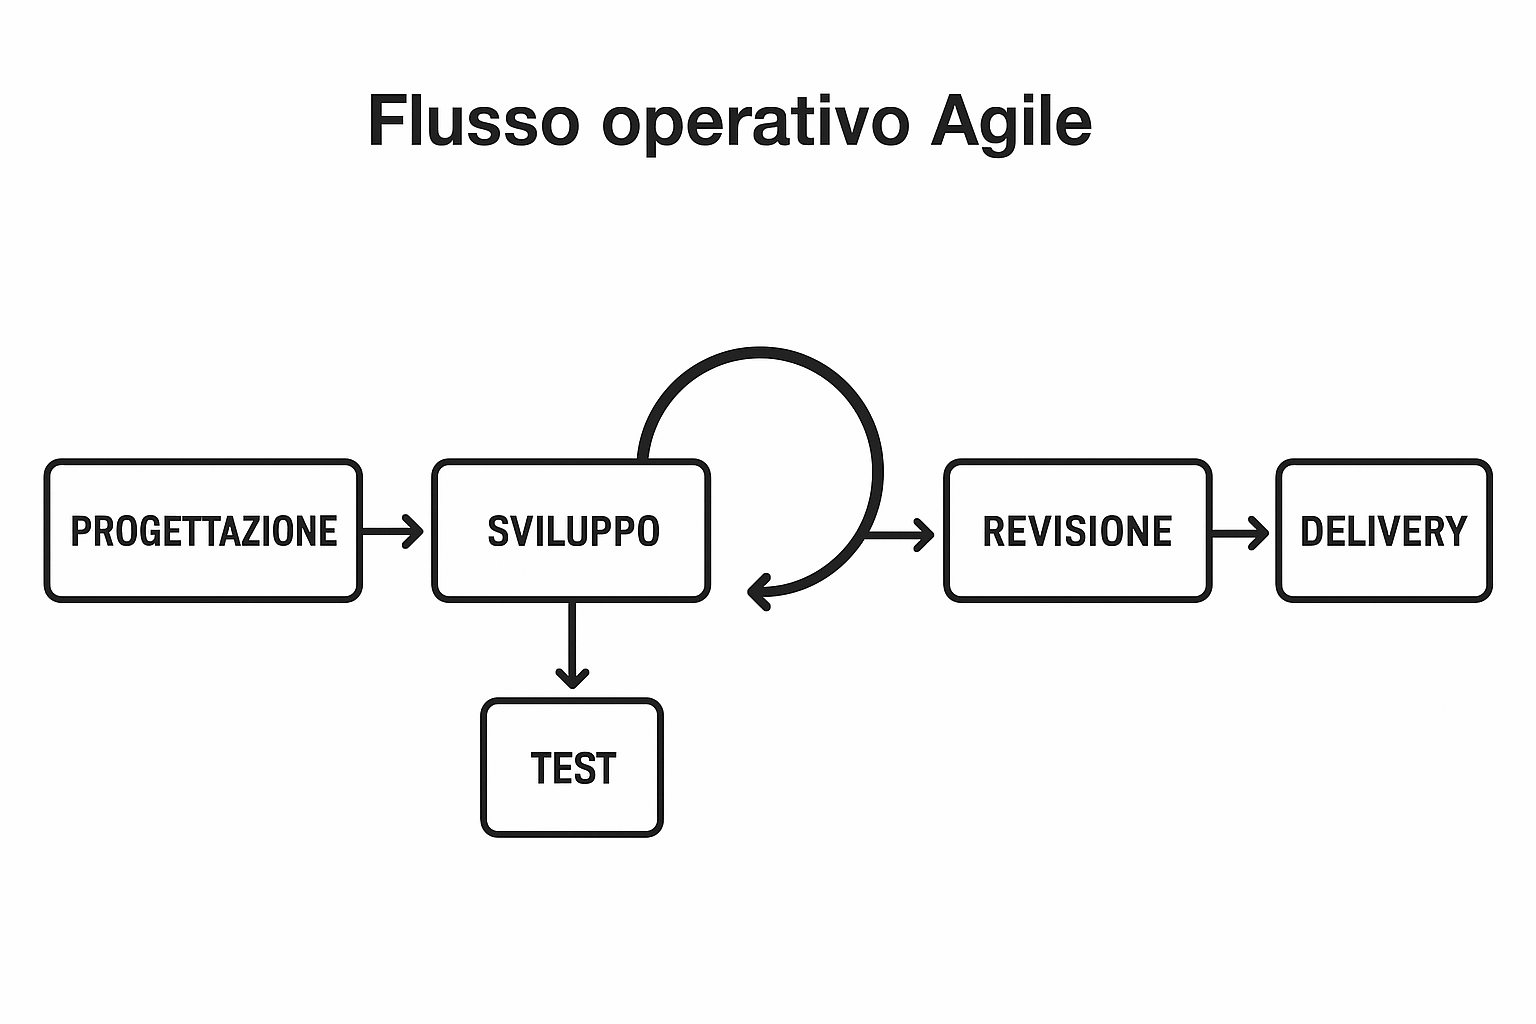
\includegraphics[width=0.8\textwidth]{images/azienda/metodo_agile.png}
    \caption{Flusso operativo Agile.}
    \label{fig:agile}
\end{figure}

Sono presenti ambienti separati per il \emph{testing} (collaudo) e per la produzione, oltre a procedure di rilascio automatizzate predisposte per i singoli progetti. 
Si alternano attività di \emph{delivery} (consegna/erogazione del servizio) su progetti custom e attività di supporto e manutenzione post-consegna.

\medskip
\noindent\textbf{Clientela}

Le informazioni sulla clientela derivano dall'analisi del sito web aziendale condotta nella fase di scelta dello stage e dall'osservazione dei progetti a cui ho partecipato. 
La clientela va dalle piccole e medie imprese con esigenze di commercio elettronico fino a grandi committenti che richiedono integrazioni complesse e soluzioni \emph{CRM} articolate. 
Sono presenti commesse nel settore privato (retail, distributori, operatori \emph{B2B}) e interventi rivolti a processi interni di organizzazioni di maggiori dimensioni.

\medskip
\noindent\textbf{Propensione all'innovazione}

La propensione all'innovazione dell'azienda è emersa chiaramente dall'analisi del progetto a me assegnato e dal modo in cui esso si è integrato nel contesto produttivo. 
Questa inclinazione si manifesta attraverso un'attenzione costante alla formazione interna, l'adozione di architetture e pratiche tecnologiche moderne e la sperimentazione su 
iniziative legate all'intelligenza artificiale. Al contempo, l'approccio rimane pragmatico: quando i vincoli operativi, i requisiti di affidabilità o i tempi di consegna lo richiedono, 
l'azienda privilegia soluzioni consolidate per garantire stabilità e robustezza.

Ho osservato una chiara divisione tra attività orientate allo sviluppo operativo e attività focalizzate sulla ricerca e sperimentazione. 
L'attività di ricerca comprende indagini tecniche per valutare nuove tecnologie e framework, lo sviluppo di \emph{proof-of-concept} (\emph{PoC}: prototipo sperimentale) e 
prototipi per dimostrare la fattibilità di idee innovative, sperimentazioni comparative e benchmark per valutare prestazioni, scalabilità e costi, oltre alla preparazione di dimostrazioni e 
documentazione tecnica da sottoporre a \emph{stakeholder} (persona o gruppo che ha interesse e influenza attività e decisioni di un'organizzazione o di un progetto).

La parte del team dedita alla ricerca crea e mette a disposizione un ambienti di sperimentazione controllato con 
branch sperimentali nel sistema di controllo versione e procedure formali per la validazione dei PoC prima di un eventuale inserimento in produzione. 

Nel complesso, la propensione all'innovazione risulta essere sia presente che ben strutturata: l'azienda favorisce l'emergere di nuove soluzioni e competenze mantenendo al contempo processi e controlli tecnici volti a 
garantire la qualità e la stabilità dei prodotti e dei servizi offerti.
\section{Obiettivi e Valori}

Sezione in cui verranno descritti gli obiettivi che l'azienda si pone con approccio innovativo nel mondo delle tecnologie nel contesto informatico e dei valori che promuove all'interno della stessa tra i colleghi.
\section{Tecnologie utilizzate}

Dal punto di vista delle piattaforme, degli strumenti operativi e delle pratiche di deployment, l’ambiente tecnologico osservato durante lo stage combina soluzioni \emph{enterprise} 
consolidate con strumenti e approcci moderni orientati alla scalabilità, all’integrazione e all’automazione. 
Di seguito viene fornita una descrizione estesa delle tecnologie principali e del loro impatto operativo.

\medskip
\noindent\textbf{\emph{Salesforce Commerce Cloud}}
\emph{Salesforce Commerce Cloud} insieme ai moduli \emph{Service Cloud} e \emph{Marketing Cloud} è una suite pensata per gestire vendite online, assistenza clienti e 
attività di marketing in modo integrato. Viene usata sia per soluzioni \emph{B2B} che \emph{B2C} e permette di costruire cataloghi prodotti, gestire ordini e mantenere 
aggiornati i profili dei clienti collegando la piattaforma ad altri sistemi aziendali (per esempio ERP, sistemi di magazzino o gateway di pagamento).
La piattaforma facilita la personalizzazione dell’esperienza d’acquisto grazie a regole commerciali e strumenti di segmentazione: è possibile mostrare contenuti, 
offerte e percorsi diversi a seconda del cliente o del canale. Allo stesso tempo automatizza molte attività di marketing e customer care (campagne, promozioni, 
follow-up post-acquisto e ticket di assistenza) riducendo lavoro manuale e tempi di risposta.

\begin{figure}[htbp]
    \centering
    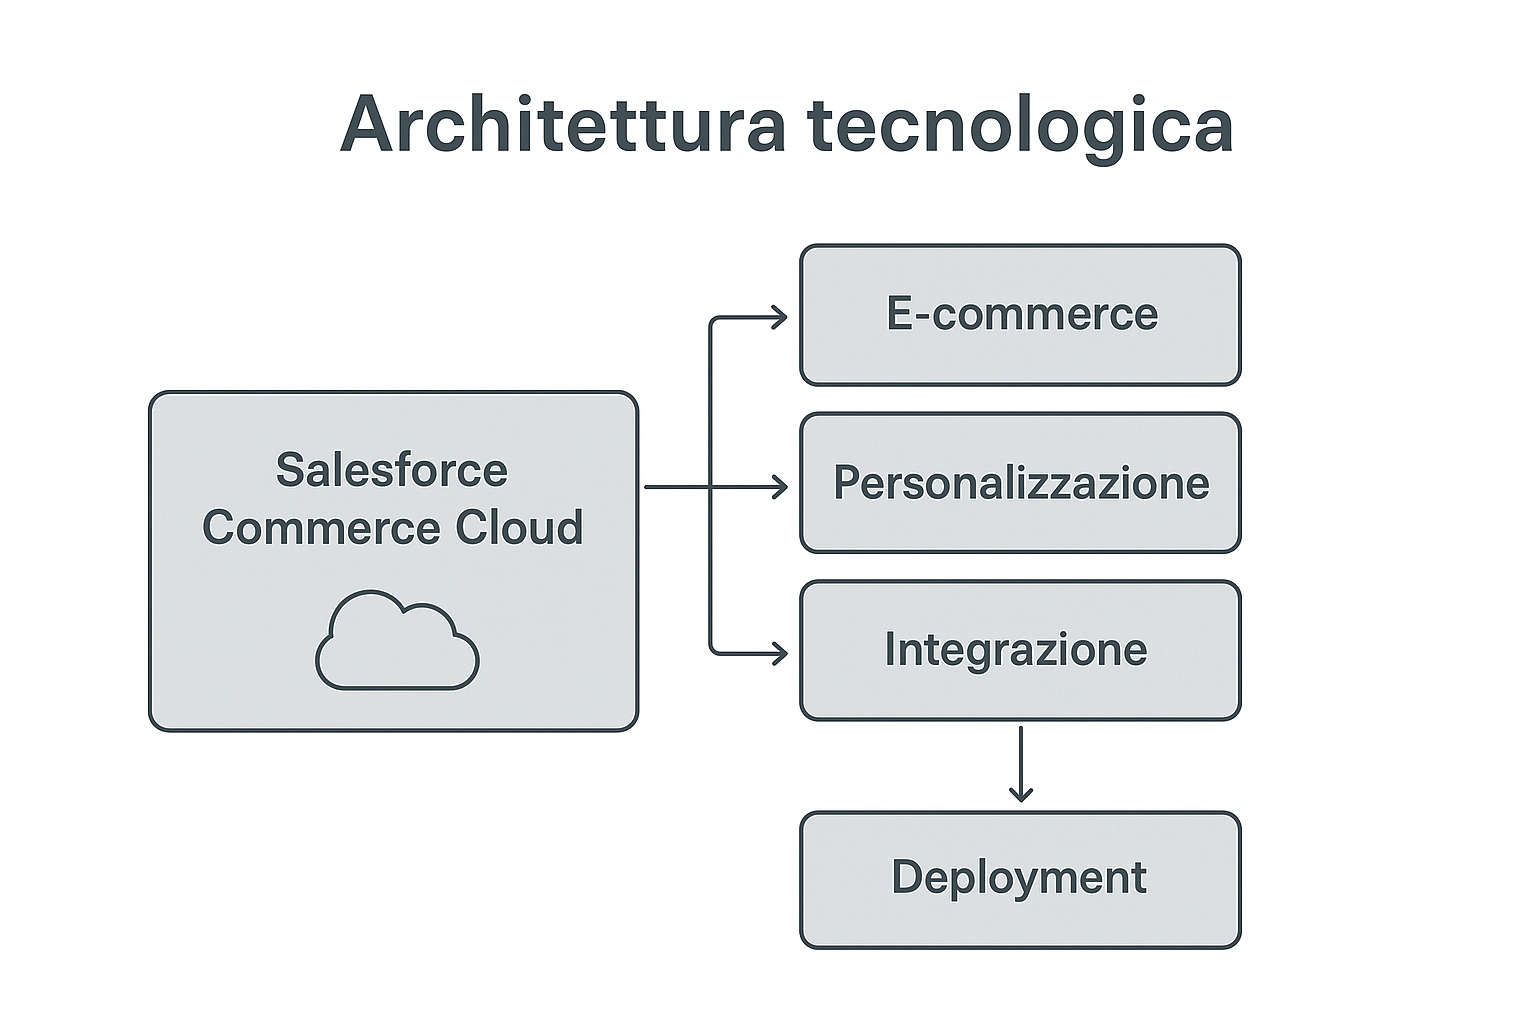
\includegraphics[width=0.8\textwidth]{azienda/architettura_tecnologica}
    \caption{Architettura tecnologica osservata: le principali piattaforme e i flussi di integrazione tra e-commerce, personalizzazione, integrazione e deployment.}
    \label{fig:architettura_tecnologica}
\end{figure}


\medskip
\noindent\textbf{\emph{Bloomreach}}
\emph{Bloomreach} è una piattaforma pensata per migliorare la ricerca interna e personalizzare la \emph{customer journey} in modo più intelligente e mirato. 
Viene impiegata soprattutto in progetti di scala per rendere le ricerche sul sito più pertinenti (per esempio mostrando risultati, suggerimenti e filtri che si adattano al contesto dell’utente) 
e per orchestrare contenuti e offerte personalizzate lungo tutto il percorso di acquisto.
Nella pratica, \emph{Bloomreach} combina segnali comportamentali, dati di prodotto e informazioni di profilo per alimentare ranking dei risultati, raccomandazioni, 
regole di \emph{merchandising} e landing page dinamiche; spesso è integrata con il \emph{CMS} (sistema per creare, gestire e pubblicare contenuti digitali senza intervento tecnico diretto) e il \emph{CRM} così da arricchire i profili utente e offrire esperienze 
realmente \emph{omnichannel} (sito, app, email e punti vendita).
I benefici tipici sono una scoperta prodotti più veloce e percorsi d’acquisto più coerenti per il cliente. Dal punto di vista operativo 
richiede però lavoro di integrazione: mappare correttamente il catalogo e i feed, definire le regole di \emph{merchandising}, impostare metriche di rilevanza e 
continuare a fare \emph{testing} per ottimizzare i risultati.

\begin{figure}[htbp]
    \centering
    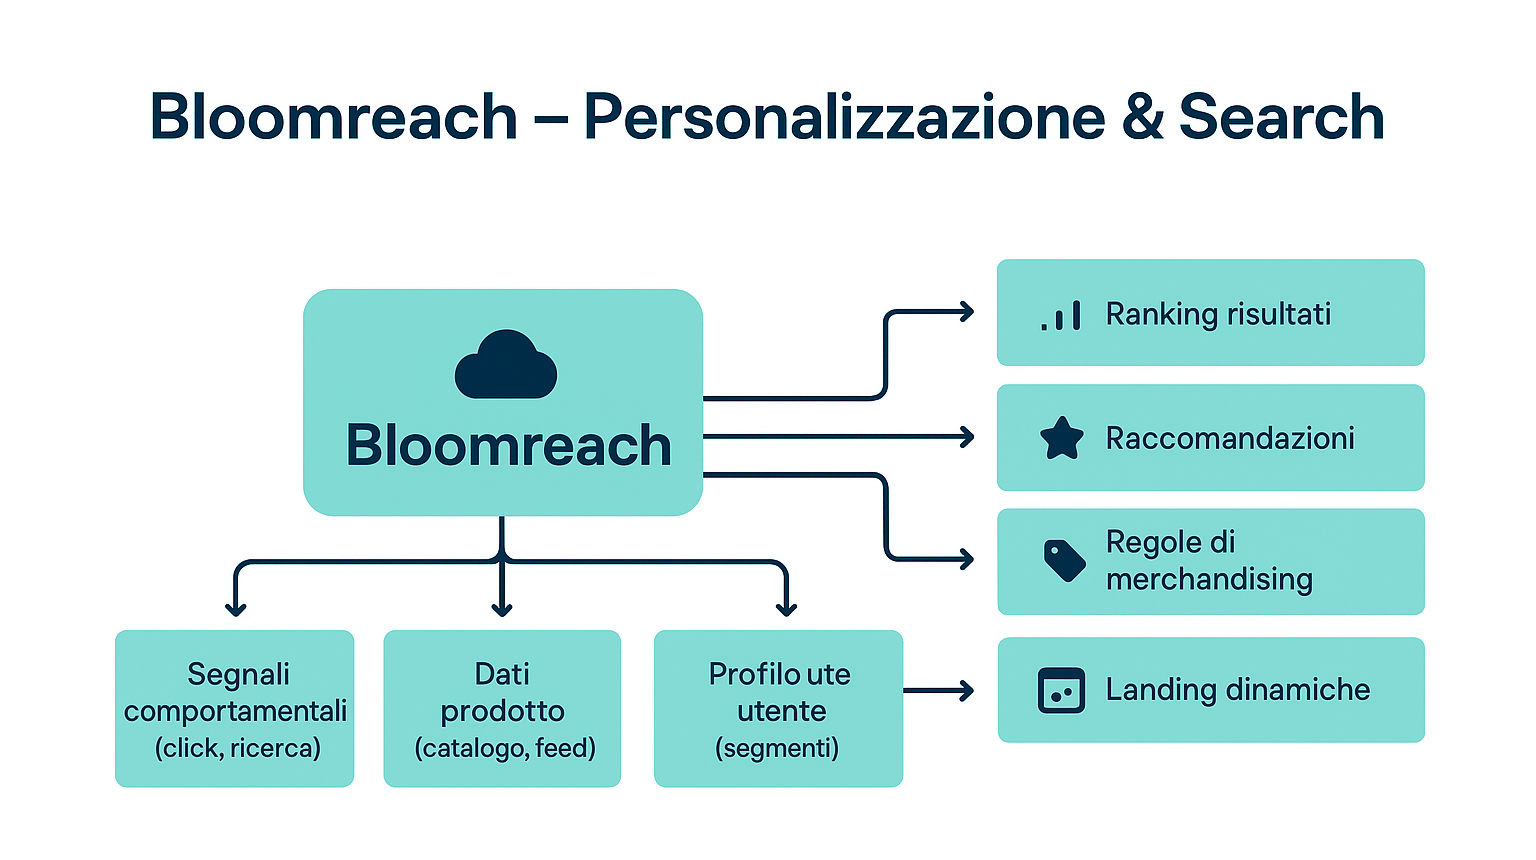
\includegraphics[width=0.8\textwidth]{azienda/bloomreach}
    \caption{Diagramma che mostra come segnali comportamentali, dati di catalogo e profili utente alimentano ranking, raccomandazioni, regole di merchandising e landing dinamiche.}
    \label{fig:bloomreach}
\end{figure}

\medskip
\noindent\textbf{\emph{deployment}}
Le piattaforme cloud e di \emph{deployment} (ad esempio \emph{AWS}, \emph{Google Cloud} e \emph{Heroku}) vengono utilizzate per ospitare le applicazioni, 
allocare risorse scalabili e creare ambienti distinti per sviluppo e collaudo (\emph{staging}) e per il traffico reale (\emph{production}). 
In pratica offrono servizi di \emph{hosting}, \emph{provisioning} delle risorse (CPU, memoria, storage) e strumenti per distribuire il codice in modo ripetibile.

Queste piattaforme sono il luogo dove risiedono i servizi applicativi, i \emph{database} e le risorse di \emph{caching}, 
e permettono di tenere separate le istanze di test da quelle in produzione per evitare impatti agli utenti. La scelta tra \emph{AWS}, \emph{Google Cloud} o \emph{Heroku} 
dipende spesso da vincoli progettuali, integrazioni richieste (per esempio con specifici servizi gestiti), competenze del team e considerazioni sui costi operativi.

Sul piano operativo si configurano meccanismi per il \emph{scaling} automatico, la distribuire del traffico, 
la gestione dei certificati \emph{TLS} per la sicurezza e sistemi di \emph{monitoring} e \emph{backup} per garantire disponibilità e resilienza. 
Inoltre si possono impostare pipeline di \emph{CI/CD} per automatizzare build, test e deployment, così da rendere le release più veloci e meno soggette a errori manuali.

Per l’infrastruttura è ormai comune l’adozione di pratiche di \emph{infrastructure as code} (strumenti che consentono il \emph{provisioning} ripetibile e tracciabile delle risorse). 

\begin{figure}[htbp]
    \centering
    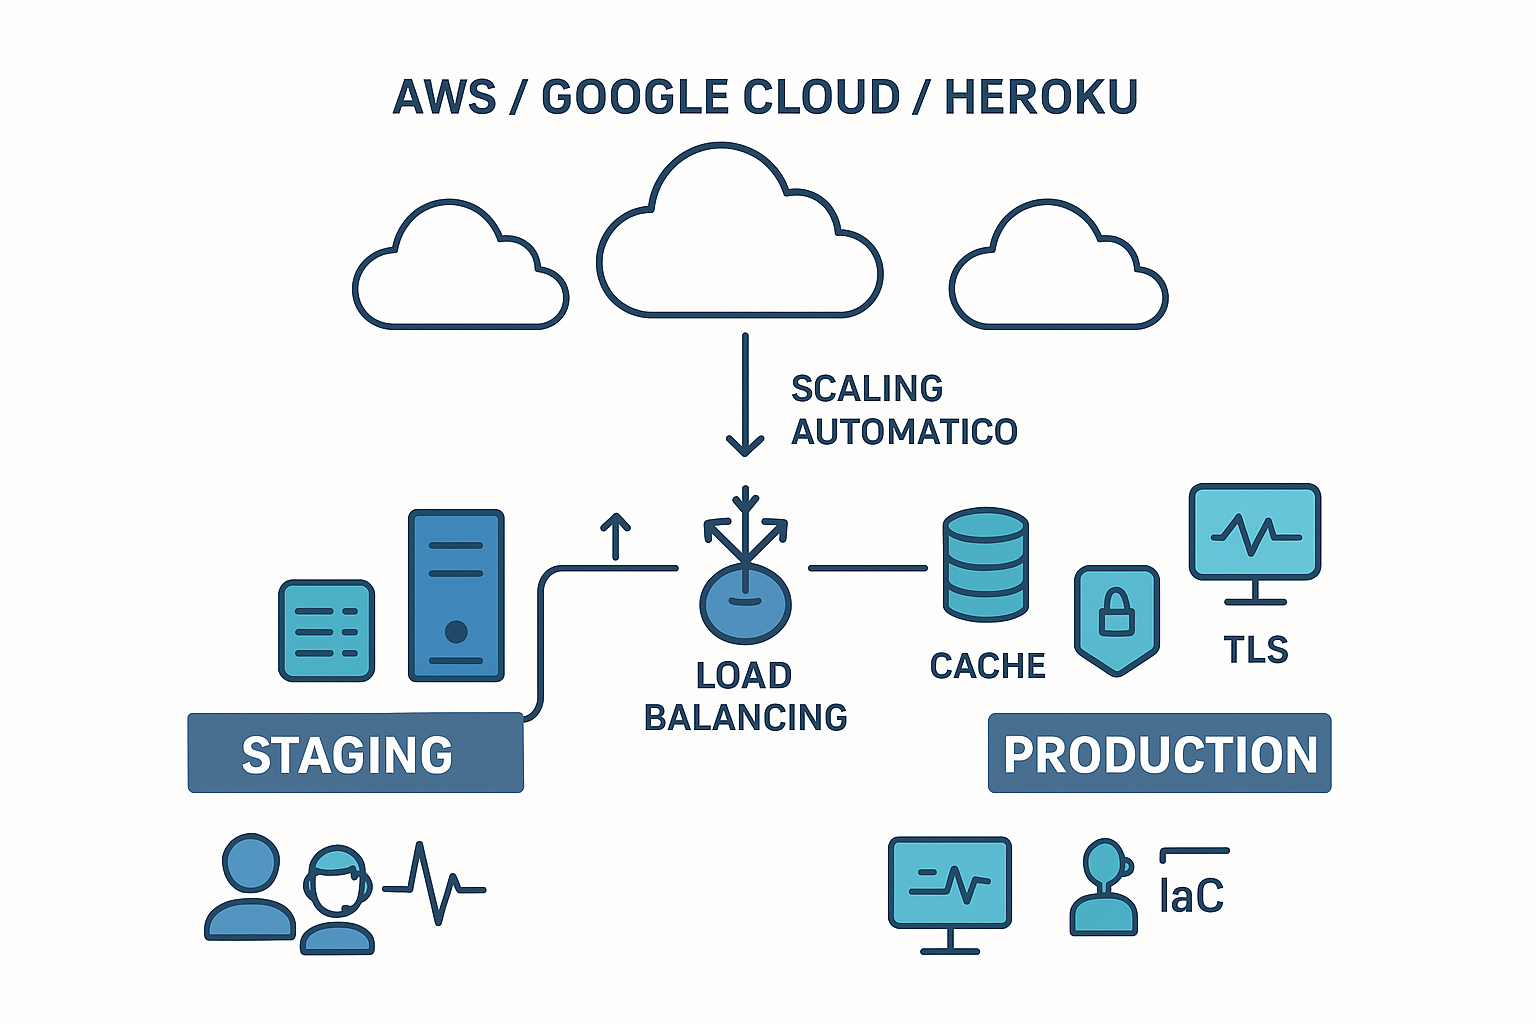
\includegraphics[width=0.8\textwidth]{azienda/deployment}
    \caption{Pipeline di integrazione e distribuzione continua: dal commit alla promozione in produzione.}
    \label{fig:deployment}
\end{figure}

% [Develop] → [Commit su Git] → [CI Build] → [Test automatici] → [Code review / Pull Request] → [Merge su main] → [Deploy su Staging] → [Verifica] → [Deploy in Production]

\medskip
\noindent\textbf{\emph{iPaaS}}
Gli strumenti di integrazione includono approcci punto a punto e soluzioni \emph{iPaaS} (\emph{Integration Platform as a Service}: piattaforme per orchestrare integrazioni) 
che collegano sistemi come \emph{CRM}, \emph{ERP}, piattaforme \emph{e-commerce} e \emph{CMS}. Mentre le integrazioni punto a punto creano connessioni dirette fra singoli sistemi, 
un \emph{iPaaS} funge da livello centrale che orchestra i flussi di dati e i processi tra più applicazioni, rendendo l'architettura più semplice da governare e manutenere.

\begin{figure}[H]
    \centering
    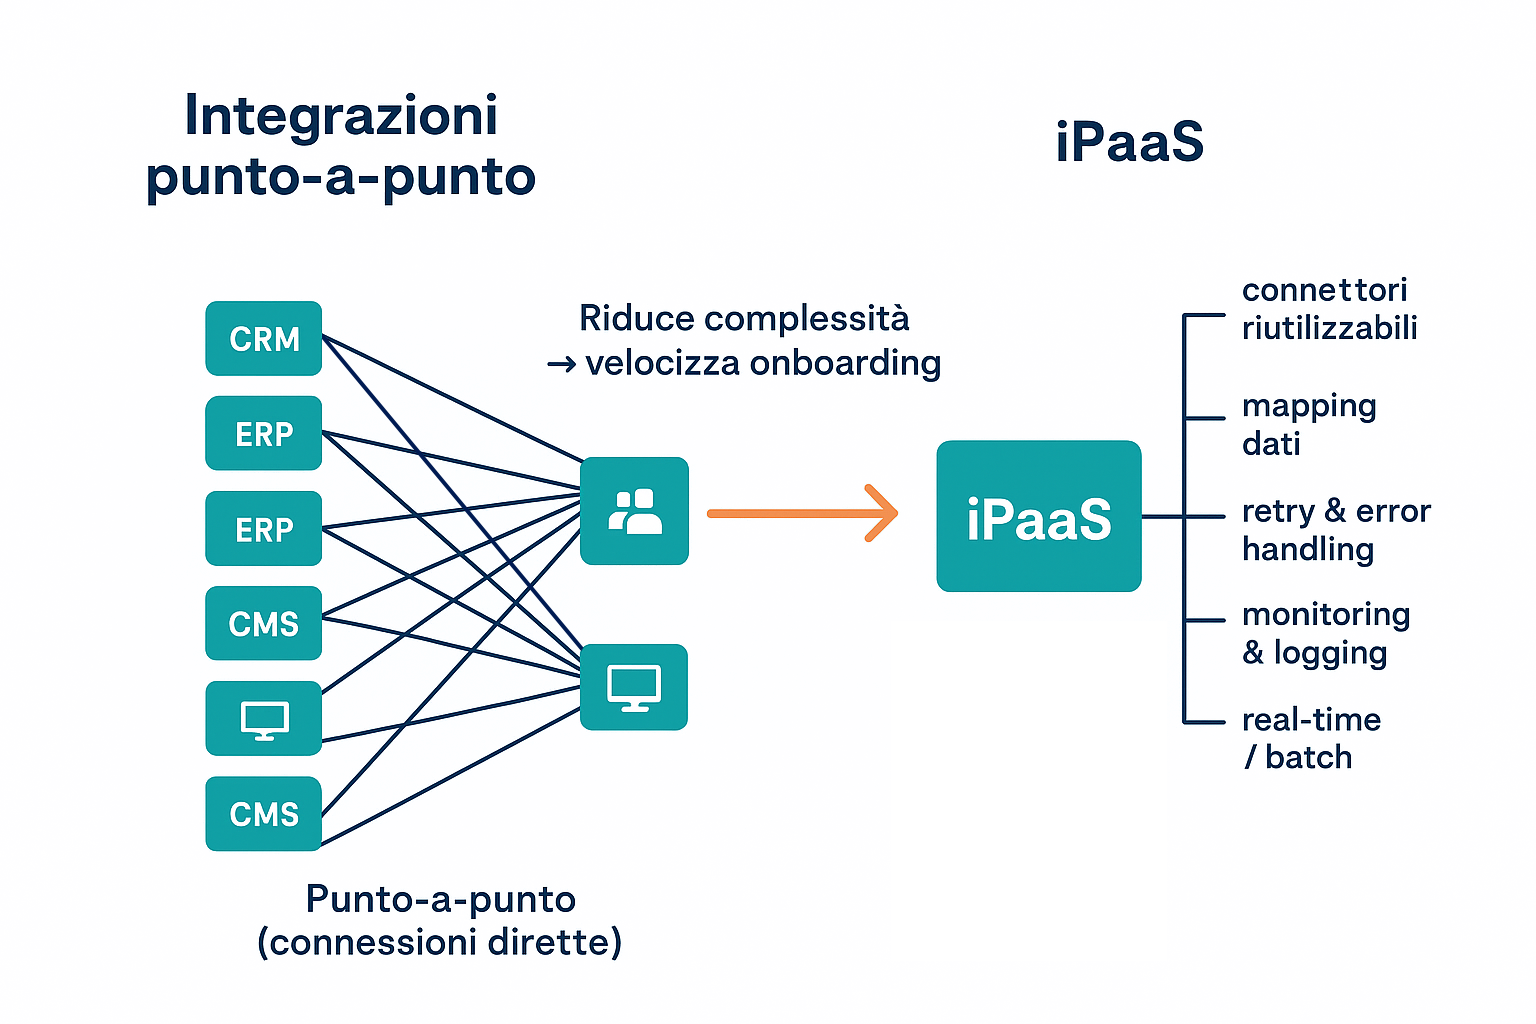
\includegraphics[width=0.8\textwidth]{azienda/iPaaS}
    \caption{Integrazioni point-to-point vs iPaaS: il diagramma mostra come un iPaaS centralizzi connettori, mapping, gestione errori e monitoring, riducendo la complessità delle integrazioni dirette e accelerando l'onboarding di nuovi sistemi.}
    \label{fig:iPaaS}
\end{figure}

L'adozione di un \emph{iPaaS} semplifica attività operative come la gestione degli \emph{endpoint} (i punti di scambio dati), la trasformazione dei \emph{payload} 
(adattamento dei formati dati), e la gestione degli errori e dei tentativi di retry (meccanismi automatici per riprovare operazioni fallite). 
Questo riduce la complessità rispetto a molte integrazioni punto a punto e velocizza l'onboarding di nuovi sistemi grazie a connettori riutilizzabili e template di integrazione.

Un \emph{iPaaS} permette anche di scegliere fra modalità di integrazione 
in tempo reale o a batch, impostare regole di mapping dei dati, e centralizzare logging e monitoraggio per individuare rapidamente problemi e colli di bottiglia.

\medskip
\noindent\textbf{Gestione progetto}
Strumenti di gestione progetto e comunicazione: \emph{Jira} per il tracciamento delle attività e \emph{Slack} per la comunicazione operativa quotidiana. \emph{Jira} 
viene usato per definire le \emph{issue} (problema, ostacolo o anomalia che richiede attenzione e risoluzione durante lo sviluppo di un progetto), assegnare priorità, documentare criteri di accettazione e tenere traccia dello stato di avanzamento; \emph{Slack} 
è lo strumento preferito per aggiornamenti rapidi e conversazioni sincrone o asincrone tra membri del \emph{team}.

\medskip
\noindent\textbf{\emph{Git}}
\emph{Git} è il fulcro del controllo versione e del coordinamento del lavoro sul codice: 
centrale non solo per conservare la storia delle modifiche, ma anche per organizzare come le nuove funzionalità arrivano nel prodotto finito. 
Nella pratica quotidiana si privilegia un flusso basato su \emph{feature branches} (ognuna per una funzionalità o correzione), 
apertura di \emph{pull request} per discutere e revisionare le modifiche (\emph{code review}) e l’uso di commit chiari e descrittivi per tracciare le decisioni.

Il processo tipico ruota attorno a poche pratiche chiave (sempre legate a \emph{Git}):
\begin{itemize}
\item sviluppo isolato su \emph{feature branches} e sincronizzazione regolare con il ramo principale per evitare divaricazioni troppo grandi;
\item revisione del codice tramite \emph{pull request} con commenti, suggerimenti e approvazioni formali prima della fusione (merge);
\item uso di convenzioni per i messaggi di commit e per i nomi dei rami (che aiutano a ricostruire la storia e a generare changelog);
\item strategie di branching consolidate (per esempio \emph{GitFlow} o approcci basati su trunk) per coordinare rilasci, hotfix e lavoro parallelo su più versioni;
\item gestione delle release tramite tag e rami dedicati alla versione (il tag identifica un punto preciso della storia come versione pubblicata);
\item pratiche di sicurezza legate a \emph{Git} (protection dei rami principali, review obbligatorie, gestione degli accessi e firma dei commit) per ridurre il rischio di errori o modifiche non autorizzate;
\item strumenti locali come le \emph{github-actions} (unità riutilizzabile di automazione che esegue compiti automaticamente in risposta a eventi del repository) e test eseguiti sul proprio ambiente prima di aprire la \emph{pull request} (ad esempio \emph{unit tests} e controlli statici), così da mantenere alta la qualità fin dal primo passo.
\end{itemize}

Dal punto di vista operativo, \emph{Git} abilita anche pratiche di rilascio sicure: le versioni vengono marcate con \emph{tag} e documentate con changelog, è possibile tornare indietro con \emph{revert} o \emph{cherry-pick} se serve correggere rapidamente una regressione, e le scelte sul tipo di merge (merge commit, fast-forward o rebase) influenzano la leggibilità della storia.

Infine, per trarre davvero vantaggio da \emph{Git} servono disciplina e coordinamento (policy per le revisioni, convenzioni condivise, role-based access) oltre a cura nella definizione dei test e nella documentazione delle release. Così, il controllo versione diventa non solo uno strumento tecnico, ma una leva organizzativa per rilasciare con più sicurezza e tracciabilità.


%\medskip

%\noindent\textbf{Implicazioni operative e suggerimenti}

%L’adozione di questo insieme di tecnologie determina alcuni vincoli e opportunità operative: la complessità delle integrazioni richiede governance dei \emph{data contracts} e 
%politiche chiare di versioning delle API; le piattaforme \emph{enterprise} come \emph{Salesforce Commerce Cloud} richiedono competenze specifiche per personalizzazioni e upgrade; 
%le risorse cloud implicano attenzione alla gestione dei costi e al monitoraggio del consumo. Per migliorare l’efficacia complessiva è raccomandabile formalizzare convenzioni comuni 
%(naming delle \emph{branches}, standard per le \emph{code review}, soglie di qualità per le \emph{pipeline}) e prevedere un minimo di documentazione operativa a supporto dell’onboarding e della manutenzione.

%In conclusione, la suite tecnologica osservata mette a disposizione strumenti potenti per costruire soluzioni integrate e scalabili; la sfida principale risiede nell’armonizzare pratiche, 
%automazioni e governance per trasformare la tecnologia in valore ripetibile e manutenibile nel tempo.


%Per la manutenzione e il supporto operativo si privilegia un approccio a livelli: monitoraggio dei servizi e dei log, 
%gestione dei \emph{ticket} tramite \emph{Jira} e interventi pianificati per aggiornamenti e patch. Nei progetti di maggiori 
%dimensioni si osserva una separazione tra team di sviluppo (feature delivery) e team di \emph{platform/operations} (monitoraggio, sicurezza, scaling), 
%mentre per clienti più piccoli le stesse persone spesso ricoprono più ruoli.

%Infine, la scelta delle tecnologie è stata chiaramente guidata dalla dimensione e dalla strategia del cliente: soluzioni \emph{Shopify} per rollout rapidi e basso \emph{TCO} 
%(\emph{Total Cost of Ownership}: costo totale di proprietà); architetture \emph{headless} e piattaforme \emph{Salesforce} per scenari enterprise e integrazioni complesse. 
%Ho inoltre riscontrato una forte propensione dell’azienda verso l’adozione di tecnologie emergenti legate all'\emph{AI} e alla personalizzazione, 
%inserite come componenti modulari (ad esempio agenti intelligenti collegati al \emph{CRM} o servizi di personalizzazione integrati con \emph{Bloomreach}). 
%In sintesi, l’ambiente tecnologico è eterogeneo e modulare, concepito per supportare sia progetti a rapido lancio sia soluzioni enterprise complesse, 
%con attenzione all’innovazione e alla scalabilità operativa.
%Sezione in cui verrà descritto il contesto produttivo in cui sono stato inserito, con particolare attenzione alle tecnologie operative viste adottare.

\section{Processi interni}

Le informazioni qui riportate derivano da osservazione diretta del mio ambiente di lavoro e da confronti brevi con il tutor interno; 
durante i due mesi di stage ho svolto il progetto in larga parte in autonomia, perciò la mia percezione dei processi si basa prevalentemente su quanto mi è stato illustrato dal tutor aziendale 
e su alcune conversazioni avute con i membri del \emph{team}, e non pretende di essere esaustiva.

\medskip
\noindent\textbf{Processo di sviluppo}

Il processo di sviluppo si articola in fasi distinte ma integrate: individuazione e definizione del problema, 
scomposizione in attività eseguibili da un solo membro del team, implementazione, verifica e rilascio. 
Per la gestione del codice e del \emph{versioning} si utilizzano strumenti dedicati (controllo di versione distribuito, repository remoti) e, 
parallelamente, si impiegano sistemi per tracciare le attività e le priorità. Dalle conversazioni tra i membri del \emph{team} ho rilevato l’esistenza di una fase iniziale di 
analisi in cui il problema viene chiarito e suddiviso in \emph{task} (attività o unità di lavoro assegnata a una persona o a un team per raggiungere un obiettivo specifico) di dimensione tale da poter essere assegnata a un singolo sviluppatore; questa scomposizione agevola la 
responsabilizzazione dei singoli e il monitoraggio dei progressi.

Lo strumento visivamente riconoscibile per la creazione, 
l’assegnazione e il monitoraggio delle \emph{tasks} è \emph{Jira}, che funge da punto di riferimento per lo stato dei lavori, le descrizioni delle attività e i commenti di avanzamento. 
Durante la fase di sviluppo giornaliera sono previste brevi \emph{stand-up meetings} (riunioni di sincronizzazione) con l’obiettivo di condividere quanto svolto nella giornata precedente, 
segnalare impedimenti e pianificare le attività immediate; queste riunioni favoriscono l’allineamento del \emph{team} e la rapida emersione di blocchi tecnici.

Al completamento di ogni \emph{task} è prevista una fase di verifica da parte di un altro membro del \emph{team} (code review): 
tale pratica viene svolta sia per assicurare qualità e conformità agli standard interni sia per favorire la diffusione delle conoscenze. 
Quando possibile, il rilascio del codice avviene seguendo procedure automatizzate che includono build e test automatici; ove presenti, 
pipeline di integrazione continua vengono attivate prima del merge verso i rami principali, riducendo il rischio di regressioni.

\begin{figure}[H]
    \centering
    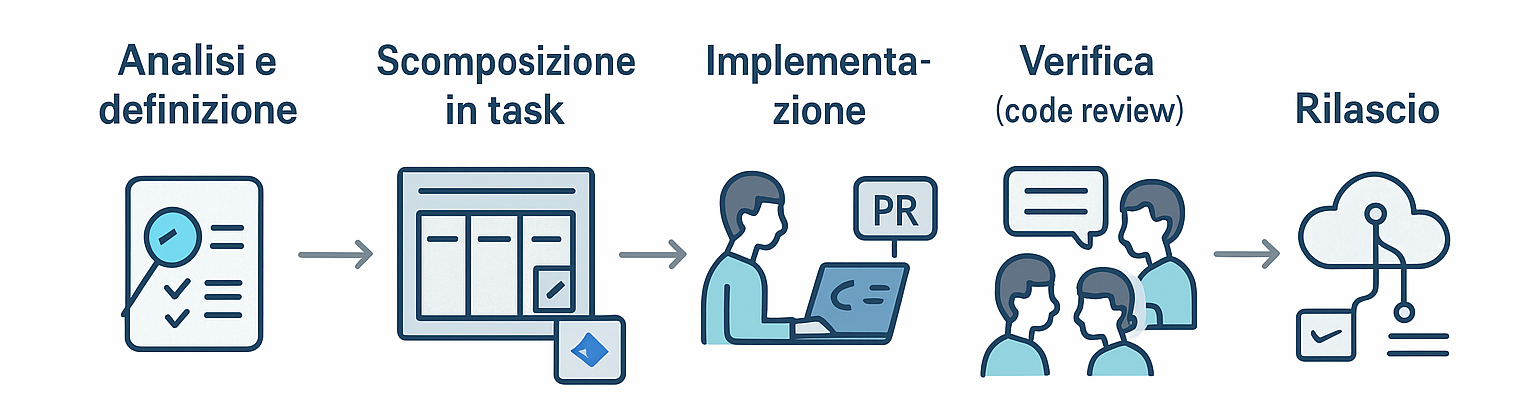
\includegraphics[width=0.8\textwidth]{azienda/processo_sviluppo}
    \caption{Flusso del processo di sviluppo adottato, dalle fasi di analisi al rilascio, con tracciamento in Jira e verifica.}
    \label{fig:processo_sviluppo}
\end{figure}

%Analisi → Scomposizione in task → Implementazione → Code review → Test → Rilascio

\medskip
\noindent\textbf{Processo di organizzazione}

L’organizzazione della comunicazione è stratificata in base al livello di formalità e alla finalità: 
comunicazioni rapide e operative avvengono su \emph{Slack}, che viene utilizzato per la pianificazione quotidiana delle presenze, richieste logistiche e notifiche veloci; 
per questioni tecniche più specifiche e per lo scambio su singole \emph{tasks} si sfruttano i \emph{branches} e i commenti collegati alle issue in \emph{Jira}, 
dove rimane tracciata la cronologia delle decisioni e delle discussioni tecniche. Le comunicazioni formali, amministrative o di carattere aziendale più strutturato vengono invece inviate tramite \emph{email}.

\begin{figure}[htbp]
    \centering
    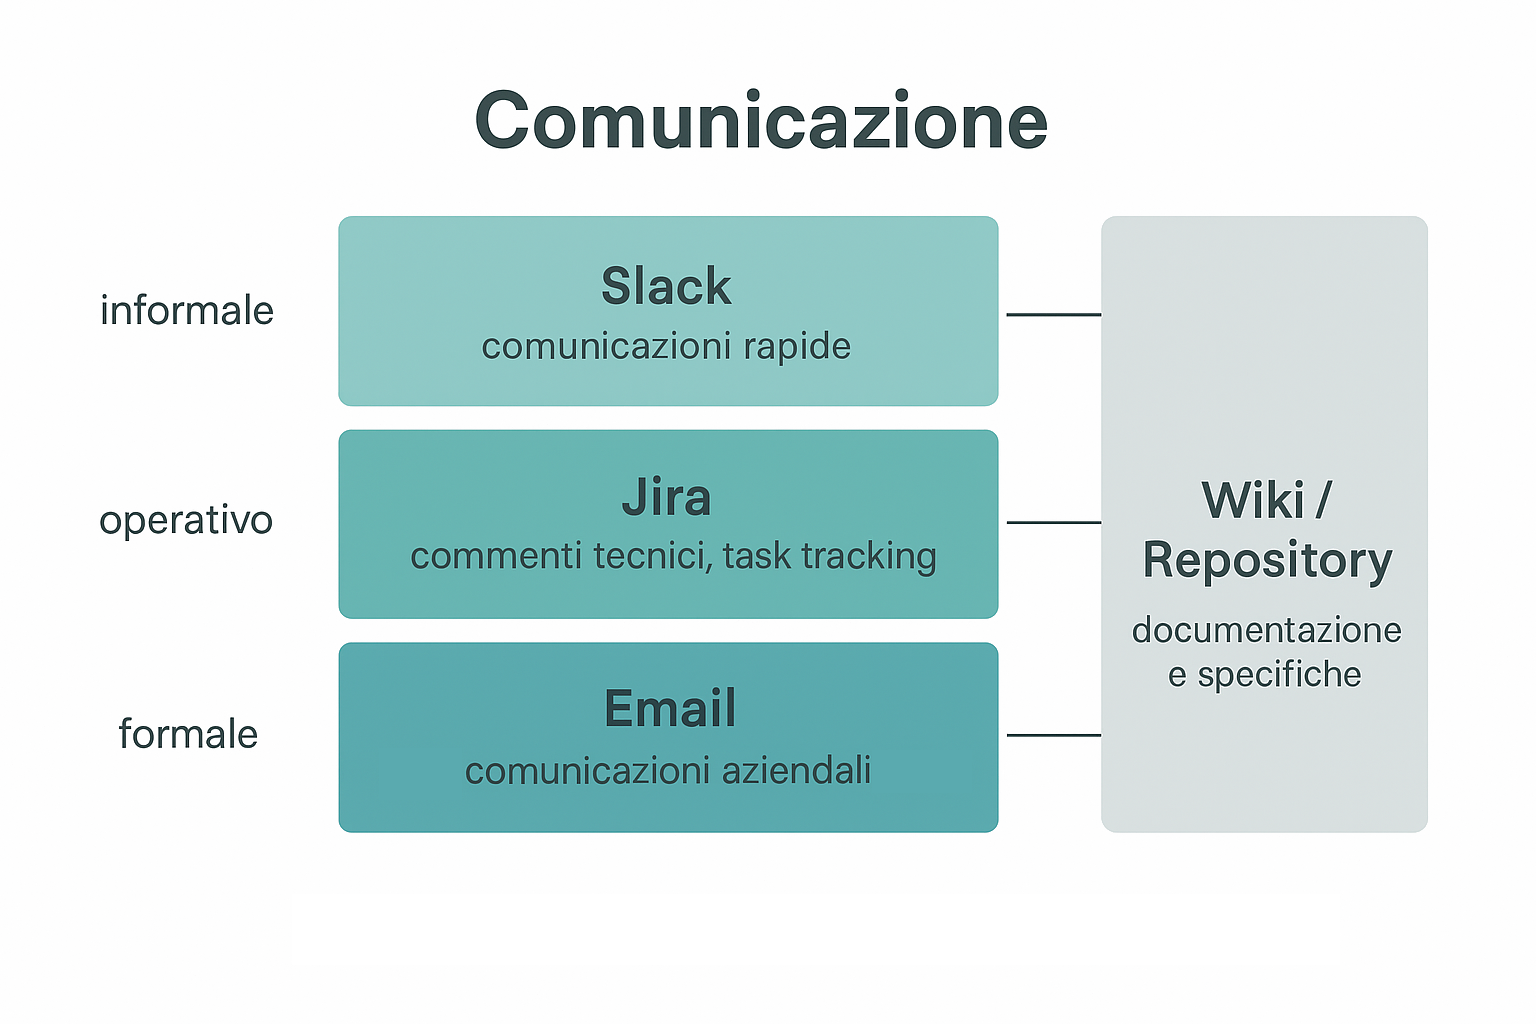
\includegraphics[width=0.8\textwidth]{azienda/comunicazione}
    \caption{Struttura dei canali di comunicazione interni e grado di formalità associato.}
    \label{fig:comunicazione}
\end{figure}

La documentazione di progetto è mantenuta in repository condivisi o in spazi dedicati (wiki, documenti di progetto): 
questo facilita il reperimento di informazioni, la consultazione delle linee guida e la storage delle specifiche. 
Ho notato che, nonostante esista una struttura di comunicazione definita, la pratica quotidiana lascia spazio a scambi informali che spesso risolvono rapidamente piccoli 
problemi ma che possono anche richiedere successiva formalizzazione quando le decisioni impattano sul piano di rilascio.

Non sono stato coinvolto nelle attività di manutenzione continuativa del sistema, né ho avuto discussioni approfondite con il tutor o con i membri del \emph{team} su procedure 
operative relative al supporto post-rilascio; pertanto non posso fornire dettagli completi su quel processo.



%Livello 1 (informale): Slack → comunicazioni rapide, Livello 2 (operativo): Jira → commenti tecnici, task tracking, Livello 3 (formale): Email → comunicazioni aziendali, amministrative, Livello trasversale: Wiki / Repository → documentazione e specifiche


%\medskip
%\noindent\textbf{Osservazioni riassuntive e suggerimenti}

%Dall’esperienza osservativa emergono alcuni punti di forza e margini di miglioramento: la presenza di pratiche consolidate (uso di \emph{Jira}, \emph{stand-up meetings}, code review) 
%favorisce trasparenza e tracciabilità, mentre l’adozione più ampia di procedure formali per la documentazione delle decisioni tecniche potrebbe ridurre la dipendenza dalle comunicazioni informali. 
%Sarebbe utile, a mio avviso, integrare nell’onboarding materiali che esplicitino il ciclo di vita di una \emph{task}, le convenzioni di \emph{versioning} adottate e le regole per le code review, 
%in modo da velocizzare l’inserimento operativo dei nuovi membri del \emph{team}.
%Processo di sviluppo:
%\begin{itemize}
%\item assegnazione delle attività tramite \emph{Jira} (strumento di gestione dei progetti e del lavoro).
%\item sviluppo locale e \emph{Versioning} con \emph{Git} (sistema di controllo versione); per i rilasci si utilizzano ambienti di prova e ambiente operativo, attivati tramite script forniti nel \emph{Repository} (archivio digitale che contiene codice, file e la cronologia delle modifiche, gestito da un sistema di versionamento);
%\item comunicazione informale prevalente su \emph{Slack} e incontri quotidiani per allineamenti ; non ho partecipato agli \emph{stand-up meetings} data la natura autonoma del mio incarico;
%\item gestione delle richieste post-rilascio tramite apertura di \emph{ticket} (voce nel sistema di tracciamento che rappresenta un'attività, un bug o una richiesta, con descrizione, stato, priorità e assegnatario) su \emph{Jira}.
%\end{itemize}

%processo di organizzazione:
%\begin{itemize}
%    \item le discussioni relative alle task (dubbi, proposte) avviene nellle sezioni relative su \emph{Jira}.
%    \item le discussioni di stampo più casuali (proposte di meeting, rchieste di conronto) avvengono tramite \emph{Slack}.
%    \item ogni comunicazione di stampo più formale non orientata ad una task nello specifico (contesto burroscratico) avviene tramite email.
%\end{itemize}

%Non sono stato coinvolto in attività legate al loro processo di manutenzione, né posso dire di averne discusso con il tutor aziendale o con i membri del team.

    \chapter{Stage}
\label{cap:stage}

\intro{Introduzione al capitolo sullo stage}\\


\section{Strategia}% e obiettivi di stage

Sezione che riporterà come lo stage si inserisce nella visione strategica da parte dell'aziendale (e dunque la  propensione dell’azienda per l’innovazione).
Qui descriverò parzialmente il punto 2 (perché) riportato nel file Struttura relazione finale.pdf. e lo concluderò nella sezione successiva.

\section{Progetto di Stage}

Sezione in cui verrà illustrato il progetto di stage ricevuto, esplicitando le problematiche applicative che l'organizzazione intende affrontare con il tirocinio, gli obiettivi specifici prefissati e i vincoli operativi e temporali associati. Verrà inoltre evidenziato il rapporto tra la proposta di stage e la strategia più ampia dell'ente ospitante in materia di innovazione — con riferimento al ruolo e alla posizione assunta dal tutor aziendale emerse nel primo incontro — nonché le attività di supporto previste prima, durante e dopo il periodo di tirocinio. Infine saranno motivate le ragioni che mi hanno portato a scegliere questa offerta rispetto ad altre.  
Qui concluderò la trattazione del punto 2 (perché) riportato nel file Struttura relazione finale.pdf.

\subsection{Descrizione Progetto}

Sotto-sezione in cui verrà descritto il progetto proposto per lo stage e perché tale idea per il progetto esista.
\subsection{Motivo della Scelta}

Sotto-sezione in cui verrà descritto il motivo per cui ho preferito scegliere di fare lo stage presso questa azienda rispetto ad altre, quali sono i miei obiettivi e come si interconnettono con gli obiettivi dell'azienda.
\section{Pianificazione}

Sezione che descriverà la pianificazione riportata nel piano di lavoro.

\subsection{Pianificazione settimanale}

\begin{tabularx}{\textwidth}{@{}l c l X@{}}
\toprule
\textbf{Settimana} & \textbf{Ore} & \textbf{Sottotitolo} & \textbf{Attività} \\
\midrule
Prima Settimana & 20 & & 
    \begin{itemize}
    \item Onboarding
    \item Accesso strumenti
    \item Revisione use case
    \end{itemize} \\

Seconda Settimana & 20 & Sottotitolo & 
    \begin{itemize}
    \item Studio tecnologie (LLM, RAG, Shopify, MCP)
    \end{itemize} \\

Terza Settimana & 20 & Sottotitolo & 
    \begin{itemize}
    \item Analisi architettura e flusso agentico
    \end{itemize} \\

Quarta Settimana & 20 & Sottotitolo & 
    \begin{itemize}
    \item Setup ambiente, primi test su API Shopify e LLM
    \end{itemize} \\

Quinta Settimana & 0--10 & Sottotitolo & 
    \begin{itemize}
    \item Pausa (ferie) o lavoro ridotto
    \end{itemize} \\

Sesta Settimana & 25 & Sottotitolo & 
    \begin{itemize}
    \item Sviluppo flusso base conversazionale
    \end{itemize} \\

Settima Settimana & 25 & Sottotitolo & 
    \begin{itemize}
    \item Integrazione RAG
    \end{itemize} \\

Ottava Settimana & 25 & Conclusione & 
    \begin{itemize}
    \item Prototipazione agent MCP
    \end{itemize} \\

Nona Settimana & 25 & Conclusione & 
    \begin{itemize}
    \item Test end-to-end conversazione $\rightarrow$ azione
    \end{itemize} \\

Decima Settimana & 25 & Conclusione & 
    \begin{itemize}
    \item Collaudo
    \item Miglioramento UX
    \item Documentazione
    \end{itemize} \\

Undicesima Settimana & 25 & Conclusione & 
    \begin{itemize}
    \item Demo finale
    \item Raccolta feedback
    \item Report
    \end{itemize} \\

\bottomrule
\end{tabularx}


%Sotto-sezione che riporterà in lista il contenuto del lavoro pianificato per lo stage, suddiviso nelle settimane definite a priori.
\subsection{Requisiti}

Sotto-sezione che riporterà la lista dei requisiti per il progetto presenti nel piano di lavoro.

\section{Metodo di lavoro}

Per lo sviluppo del progetto, in accordo con il tutor aziendale, è stata adottata una modalità di lavoro ibrida: 1–2 giorni alla settimana in presenza e il resto in remoto, 
con l'obiettivo di integrarmi nell'ambiente del \emph{team} che utilizza la stessa organizzazione. Per la comunicazione sincrona e asincrona ho impiegato 
\emph{Slack} per le interazioni quotidiane col tutor aziendale (richieste di chiarimenti, notifiche di avanzamento, condivisione di link e documenti) e per confermare i giorni di presenza 
della settimana successiva; per il lavoro in presenza ho utilizzato il mio PC portatile predisposto con l'ambiente di sviluppo richiesto dal progetto.

Il metodo di lavoro è stato concordato con il tutor aziendale attraverso un confronto iniziale e successive definizioni condivise: alcune parti del 
flusso mi sono state illustrate, altre sono state discusse e adattate tenendo conto delle mie osservazioni e competenze. Il processo complessivo è stato organizzato 
in fasi sequenziali e iterative; per ogni fase era previsto il rilascio di uno o più artefatti documentali e/o \emph{software} a supporto della valutazione e della 
verifica da parte del tutor aziendale. In particolare i \emph{deliverables} richiesti sono stati: documento di analisi del dominio (dimostrato anche tramite un \emph{playground} 
personale con esperimenti sulle tecnologie), documento di scelta tecnologica, specifica tecnica per il \emph{Proof of Concept} (\emph{PoC}) e la \emph{repository} ordinata 
con relativo \texttt{\emph{README.md}}.

\begin{figure}[H]
    \centering
    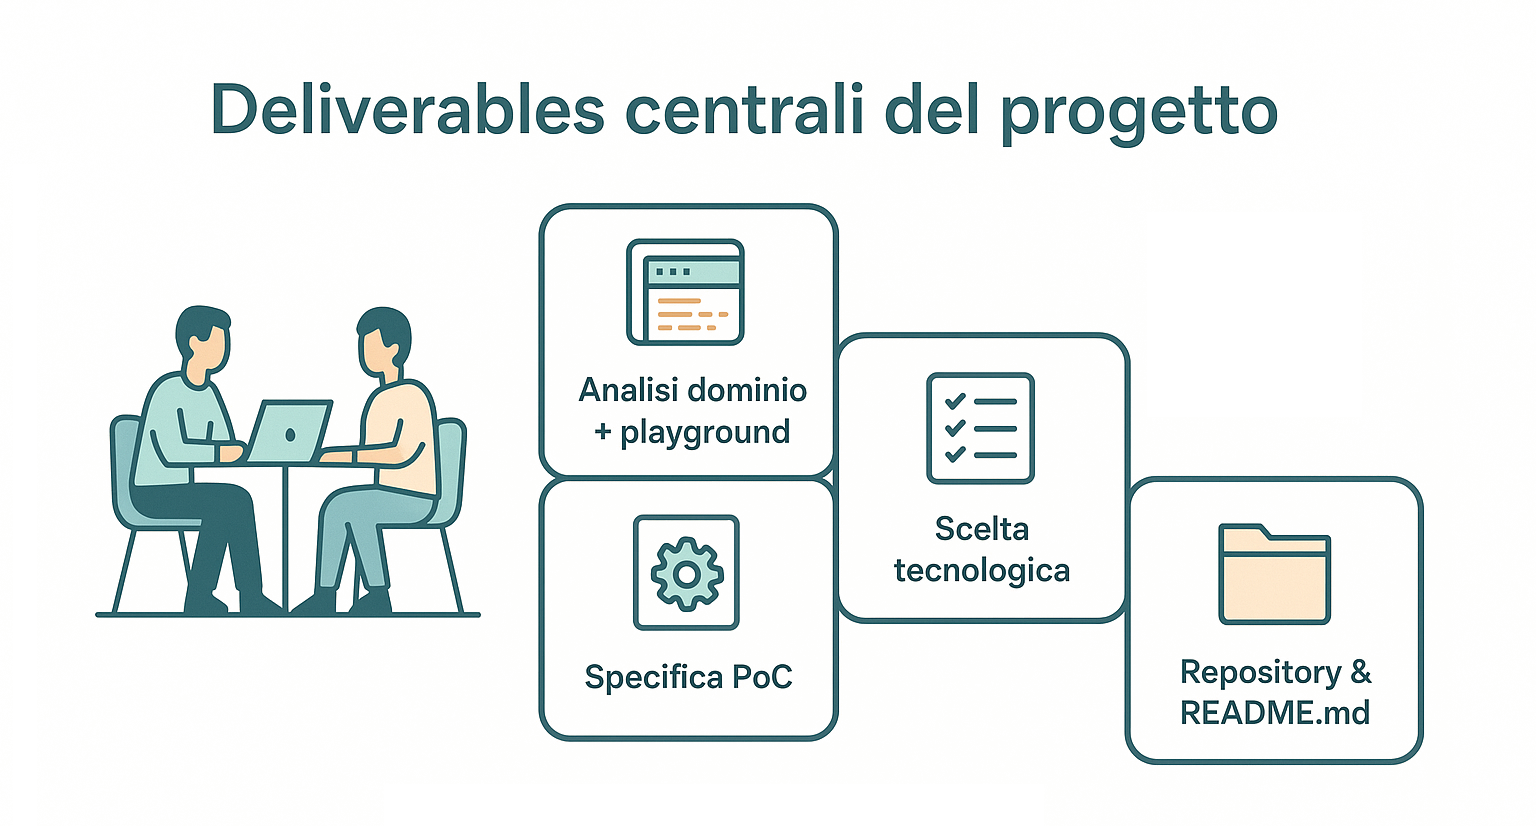
\includegraphics[width=0.8\textwidth]{stage/metodo}
    \caption{Schema del metodo di lavoro adottato.}
    \label{fig:metodo}
\end{figure}

Per garantire controllo, tracciabilità e qualità, ho seguito le pratiche sotto elencate, applicandole coerentemente alle attività giornaliere e alle revisioni settimanali:

\medskip
\noindent\textbf{Pianificazione e gestione delle attività}
Il progetto è stato pianificato in \emph{milestone} e \emph{task}: ogni \emph{milestone} conteneva obiettivi funzionali chiari e criteri di accettazione. 

\medskip
\noindent\textbf{Interazioni e revisioni con il tutor aziendale}
È stata stabilita una cadenza settimanale di incontro (giorno concordato di settimana in settimana) in cui presentare i progressi; 
ogni riunione seguiva un ordine del giorno strutturato: stato di avanzamento, dimostrazione pratica (se applicabile), punti aperti e rischi e proposte di soluzione.

\medskip
\noindent\textbf{Tracciamento dei requisiti e tecniche di analisi}
Ho adottato una procedura di tracciamento dei requisiti che mantenesse la relazione tra requisiti, attività di sviluppo e \emph{test}. 
Questo è stato realizzato tramite una semplice matrice di tracciabilità che associa ad ogni requisito: descrizione, priorità, \emph{task}/\emph{issue} corrispondenti.

\medskip
\noindent\textbf{Controllo della qualità del software e strumenti di verifica}
Per il codice ho seguito pratiche consolidate: utilizzo di controllo versione 
(\emph{git}) con flusso a \emph{feature-branch} e \emph{linters/formatter} per mantenere qualità e uniformità. 
Ho predisposto \emph{test} manuali per i componenti critici, per le \emph{API} e le varie integrazioni. 
Per la verifica funzionale del PoC sono stati definiti casi di \emph{test} che verificano il rispetto dei requisiti definiti nel relativo documento.

\medskip
\noindent\textbf{Sicurezza e gestione dei dati}
Per le integrazioni con \emph{API} esterne (Shopify e Sanity) e per qualsiasi dato sensibile ho rispettato accorgimenti base: 
uso di variabili d'ambiente, non salvataggio di chiavi in chiaro e repository privata con accesso consentito solamente al tutor aziendale.

\medskip
\noindent\textbf{Documentazione e repository}
La repository del progetto è stata organizzata con una struttura logica (cartelle per codice, \emph{test} e documentazione) 
e corredata da un \texttt{\emph{README.md}} esaustivo che spiega come eseguire il progetto, come riprodurre il \emph{PoC} e quali sono i componenti principali.


%interazioni con il tutor aziendale



%Sezione che riporterà il flusso di lavoro uilizzato per lo sviluppo del progetto in accordo con il tutor aziendale.
%Verranno riportati pianificazione, interazioni con il tutor aziendale, revisioni di progresso, uso di diagrammi,
%tecniche di analisi e tracciamento dei requisiti, strumenti di verifica, ecc.
%Qui descriverò il punto 3.a (cosa e come) riportato nel file Struttura relazione finale.pdf.


\section{Tecnologie utilizzate}

Il progetto si è basato sulla realizzazione di un \emph{PoC} volto a migliorare la fruibilità mediante un flusso agentico del servizio offerto da \emph{Comfortzone}. 
Essendo il servizio di \emph{e-commerce} di \emph{Comfortzone} oggetto di \emph{re-breanding} da parte dell'azienda ospitante, si è deciso di adottare alcune tecnologie 
ritenute necessarie per il loro sito, tra cui \emph{Sanity} come \emph{CMS} e \emph{Shopify} per la gestione delle operazioni di commercio elettronico.

\subsection{Sanity}

La scelta di adottare \emph{Sanity} come \emph{Content Management System (CMS)} sarebbe stata dettata dalla necessità di gestire in modo strutturato e flessibile le informazioni aziendali, 
rendendole facilmente accessibili a uno o più agenti intelligenti coinvolti nel progetto. 
In particolare, l’obiettivo sarebbe stato quello di mettere a disposizione dell’agente un corpus di conoscenze coerente, aggiornato e contestualizzato rispetto ai 
contenuti pubblicati da \emph{Comfortzone}, così da garantire risposte più affidabili e pertinenti alle richieste degli utenti.

\emph{Sanity} si sarebbe rivelato particolarmente adatto per la sua natura \emph{headless}, che avrebbe consentito di separare la gestione dei contenuti dalla loro 
presentazione e di esporre i dati tramite \emph{API} dedicate. Tale caratteristica avrebbe permesso di integrare facilmente articoli del \emph{blog}, 
schede prodotto e pagine informative in un backend accessibile programmaticamente, favorendo l’estrazione selettiva di informazioni attraverso query mirate (\emph{GROQ}) e 
sperimentazioni in ambiente di \emph{playground}.

Sfruttando il \emph{playground} e le \emph{API}, sarebbe stato possibile testare diverse strategie di estrazione, chunking e indicizzazione dei contenuti per valutare la soluzione più 
efficace per il retrieval semantico dell’agente. Inoltre, la gestione di metadati e riferimenti tra documenti avrebbe facilitato la creazione di segnali utili al ranking e alla 
ricostruzione del contesto nelle risposte generate.

Dal punto di vista operativo, l’utilizzo di \emph{Sanity} avrebbe garantito anche un vantaggio pratico: i team editoriali avrebbero potuto aggiornare i contenuti in autonomia e in tempo reale, 
riducendo la necessità di interventi tecnici e assicurando che le conoscenze a disposizione dell’agente rimanessero allineate con le pubblicazioni ufficiali. Questa flessibilità, 
unita alla facile integrazione con servizi esterni (ad es. pipeline per la generazione di embedding o webhook per la sincronizzazione), avrebbe reso \emph{Sanity} 
coerente con gli obiettivi di sperimentazione rapida, scalabilità e iterazione tipici di un \emph{Proof of Concept}.

In sintesi, \emph{Sanity} avrebbe offerto un equilibrio tra struttura dei contenuti, accessibilità via \emph{API} e praticità operativa, elementi che si sarebbero rivelati 
utili per supportare l’agente conversazionale e le successive valutazioni sul suo impatto funzionale e strategico.

\subsection{Shopify}

La scelta di \emph{Shopify} è stata motivata dalla necessità di disporre di una piattaforma e-commerce robusta, già adottata dall'azienda, che permettesse 
sia la presentazione dei prodotti agli utenti sia la gestione operativa degli stessi dallo store. Nel PoC si è quindi previsto un'integrazione che coprisse due bisogni principali: 
(i) mostrare in modo consistente i prodotti presenti nello \emph{store} tramite uno \emph{storefront} accessibile all'agente e all'interfaccia utente; 
(ii) permettere aggiornamenti lato \emph{store} relativi a prezzo, disponibilità e metadati quando necessario.

Di seguito vengono descritti i dettagli tecnici e le scelte adottate nell'integrazione con \emph{Shopify}, 
le responsabilità dei vari componenti e le scelte progettuali per garantire sicurezza, performance e tracciabilità.

Architettura di integrazione e API utilizzate — l'integrazione con Shopify è stata realizzata su due livelli distinti ma coordinati:
\begin{itemize}
\item \textbf{Storefront API (client-side)}: utilizzata per operazioni che devono avvenire direttamente dal cliente/utente o dall'agente in tempo reale, 
come la visualizzazione di catalogo, interrogazioni sui prodotti, recupero di varianti e operazioni sul carrello (aggiungi/rimuovi articoli, aggiornamento quantità). 
Questo approccio permette all'interfaccia lato client e agli agenti conversazionali di effettuare operazioni con latenza minima e senza esporre privilegi di amministrazione.
\item \textbf{Admin API / private app / app server (server-side)}: utilizzata per le operazioni di aggiornamento dello store 
(creazione o aggiornamento di prodotti, modifiche di prezzo, gestione inventario, modifica di metafields). 
Queste operazioni richiedono token con scope elevati e quindi sono eseguite tramite un backend protetto (server o funzione serverless) che espone endpoint sicuri verso il \emph{PoC}. 
Tutte le chiamate di scrittura passano per questo \emph{layer} di \emph{backend} per proteggere le credenziali e implementare logica aggiuntiva (validazione, trasformazione dati, \emph{audit}).
\end{itemize}

Autenticazione, scope e gestione dei segreti — i token con privilegi di scrittura non sono mai esposti al client. Nel \emph{PoC} si è adottata la seguente politica:
\begin{itemize}
\item uso di token lato server conservati in variabili d'ambiente e, in ambiente aziendale, in secret manager o vault aziendali;
\item uso di token a lettura limitata per eventuali integrazioni serverless con privilegi minimi;
\item gestione del flusso OAuth (se necessario per app pubbliche) o app private per development store, con rotazione dei token e log delle operazioni di amministrazione.
\end{itemize}

Mapping dei dati e coerenza con il CMS — per permettere all'agente di correlare catalogo e contenuti editoriali (gestiti da \emph{Sanity}) è stata definita una strategia di mapping:
\begin{itemize}
\item utilizzo di campi identificativi condivisi (SKU, handle/slug, metafields) per collegare entità in Shopify con documenti in Sanity;
\item sincronizzazione o arricchimento dei dati mediante pipeline: quando un prodotto viene aggiornato in Shopify (es. variazione prezzo o disponibilità) un \emph{webhook} notifica 
il \emph{backend} che aggiorna l'indice usato dall'agente; viceversa, modifiche nei contenuti editoriali in Sanity possono popolare metafields utili per display o per guide prodotto.
\end{itemize}

Webhooks, sincronizzazione e strategie di aggiornamento — per mantenere coerenza e ridurre latenza tra store e PoC si sono sfruttati i webhooks (publish/updated/delete/inventory) di Shopify:
\begin{itemize}
\item i webhooks innescano pipeline di aggiornamento che normalizzano il payload, aggiornano l'indice di ricerca o il database di riferimento e rigenerano eventuali 
\emph{embedding} se questi dati sono parte del knowledge base;
\item per campi critici (prezzi, stock) si è privilegiata la notifica push via webhook e l'interrogazione puntuale dell'Admin API in caso di necessità di conferma.
\end{itemize}

Operazioni sul carrello e limiti client — l'agente e l'interfaccia utente devono poter svolgere operazioni sul carrello. Queste funzionalità sono state implementate 
principalmente tramite Storefront \emph{API}, rispettando i seguenti vincoli:
\begin{itemize}
\item le operazioni di manipolazione del carrello (add/remove/update) avvengono lato client o tramite endpoint serverless che mediano le chiamate, preservando la sicurezza;
\item il completamento dell'ordine (checkout e pagamento) non è stato automatizzato dal PoC per motivi di sicurezza e compliance: il flusso prevede la redirezione dell'utente 
al \emph{checkout} \emph{Shopify} o l'uso di un \emph{checkout} protetto, lasciando la transazione finale all'infrastruttura \emph{Shopify}.
\end{itemize}

Gestione delle varianti, prezzi e disponibilità — i prodotti in Shopify possono avere varianti con stock e prezzi differenti; per gestire questo:
\begin{itemize}
\item l'agente identifica e presenta le varianti rilevanti (es. colore, taglia) esponendo SKU e attributi utili per la scelta;
\item il PoC prevede la risoluzione dei conflitti di prezzo leggendo i prezzi correnti dallo store in tempo reale quando la freschezza è critica;
\item per la visualizzazione viene mantenuta una cache controllata per non saturare le API e per migliorare le prestazioni (TTL impostato in base alla volatilità dei dati).
\end{itemize}

Caching, performance e limiti di rate — per ottimizzare prestazioni e costi si sono adottate politiche di caching lato server e client, con invalidazione guidata da eventi (\emph{webhook}). 
Inoltre sono state previste logiche di backoff e retry per rispettare i limiti di rate delle API di Shopify e ridurre errori transienti.

Testing, monitoraggio e qualità — il PoC ha previsto attività di validazione su due livelli:
\begin{itemize}
\item \textbf{testing automatico e manuale}: test di integrazione che verificano chiamate all'API (mockate in ambiente di sviluppo),
 test di end-to-end sui flussi di aggiunta al carrello e sulla corretta risoluzione di varianti; uso di strumenti per l'invocazione automatizzata di endpoint 
 (es. Postman/Newman o test automatizzati);
\item \textbf{monitoraggio e logging}: tutte le operazioni di scrittura sono state loggate con ID di correlazione per tracciare cambiamenti e agevolare debug; 
alert su errori critici e metriche di successo delle webhook callback.
\end{itemize}

Sicurezza, privacy e conformità — considerata la natura dei dati trattati, nel PoC sono state seguite pratiche conservative:
\begin{itemize}
\item non memorizzare dati sensibili degli utenti nei log (sanitizzazione);
\item conformità alla normativa sulla protezione dei dati nel trattamento di eventuali informazioni personali usate nei test (dati sintetici o anonimizzati);
\item criteri di accesso basati sul principio del minimo privilegio.
\end{itemize}

Limitazioni e mitigazioni — durante lo sviluppo del PoC sono emerse limitazioni da considerare:
\begin{itemize}
\item alcune operazioni amministrative possono richiedere permessi non replicabili in ambienti di produzione senza una review; per questo il PoC ha privilegiato 
l'uso di ambienti di sviluppo o store di test per le scritture;
\item la sincronizzazione bidirezionale tra CMS e store può generare condizioni di race: si sono introdotte politiche di reconciliation, timestamping e idempotenza per mitigare conflitti;
\item il completamento dei pagamenti e la gestione di transazioni reali sono stati lasciati alla piattaforma Shopify per motivi di sicurezza e compliance.
\end{itemize}

Integrazione con l'agente conversazionale — infine, l'interazione dell'agente con Shopify è stata progettata per massimizzare utilità e sicurezza:
\begin{itemize}
\item l'agente può interrogare il catalogo (filtri, ricerca semantica assistita da indici vettoriali) e proporre prodotti coerenti con la conversazione;
\item può costruire e modificare un carrello virtuale per mostrare all'utente l'impatto di scelte diverse, ma la persistenza finale e il checkout rimangono operazioni gestite dal backend/Shopify;
\item tutte le risposte che coinvolgono dati sensibili (prezzi speciali, stock limitati, promozioni) richiedono conferma tramite meccanismi server-side prima di essere applicate allo store.
\end{itemize}

In sintesi, l'adozione di \emph{Shopify} nel PoC ha consentito di sfruttare una piattaforma e-commerce matura per la presentazione e la gestione del catalogo, garantendo al tempo 
stesso che le operazioni critiche siano eseguite in modo sicuro tramite un livello server-side. La combinazione fra Storefront API per le interazioni in tempo reale e Admin API 
per le operazioni di aggiornamento, integrata con webhooks, caching e politiche di sicurezza, ha permesso all'agente di offrire funzionalità utili all'utente senza compromettere 
la sicurezza o la consistenza dei dati nello store.


%Sotto-sezione che riporterà la spiegazione e la logica della scelta delle API di Shopify.

    \chapter{Analisi dei Requisiti}
\label{cap:analisi-requisiti}

\intro{Introduzione al capitolo sull'analisi dei requisiti}\\

\section{Use Case}

\subsection{UC-1: Interazione tra utente e agente IA}

Descrizione dettagliata del Use Case UC-1.

\subsection{UC-2: Aggiungi prodotto al carrello}

Descrizione dettagliata del Use Case UC-2.

\subsection{UC-3: Elimina prodotto dal carrello}

Descrizione dettagliata del Use Case UC-3.

\subsection{UC-4: Modifica prodotto nel carrello}

Descrizione dettagliata del Use Case UC-4.

\subsection{UC-5: Prepara al check-out}

Descrizione dettagliata del Use Case UC-5.

\subsection{UC-6: Visualizza errore nell'uso di un tool}

Descrizione dettagliata del Use Case UC-6.

\subsection{UC-7: Richiesta informazioni sul contenuto del carrello}

Descrizione dettagliata del Use Case UC-7.

\subsection{UC-8: Richiesta informazione specifica su un prodotto nel catalogo}

Descrizione dettagliata del Use Case UC-8.

\subsection{UC-9: Visualizza spiegazione di una possibile routine con i prodotti nel carrello}

Descrizione dettagliata del Use Case UC-9.

\subsection{UC-10: Visualizza proposta per un prodotto in coerenza con quelli nel carrello}

Descrizione dettagliata del Use Case UC-10.

\subsection{UC-11: Visualizza il log dei messaggi}

Descrizione dettagliata del Use Case UC-11.

\subsection{UC-12: Visualizza contenuto in output in lingua specifica}

Descrizione dettagliata del Use Case UC-12.

\section{Requisiti}

\subsection{Obbligatori}

Contenuto dei requisiti obbligatori.

\subsection{Facoltativi}

Contenuto dei requisiti facoltativi.


    \chapter{Sviluppo}
\label{cap:sviluppo}

\intro{Introduzione al capitolo sullo sviluppo}\\

\section{Tecnologie utilizzate}


\subsection{Fast-api}

Sotto-sezione che riporta la spiegazione e la logica della scelta del framwork Fast-api.
\subsection{Gemini}

Sotto-sezione che riporta la spiegazione e la logica della scelta dell'LLM Gemini.
\subsection{Google-adk}

Sotto-sezione che riporta la spiegazione e la logica della scelta del framwork Google-adk.
\subsection{Hydrogen}

Sotto-sezione che riporterà la spiegazione e la logica della scelta del framwork Hydrogen.
\subsection{Pinecone}

Sotto-sezione che riporta la spiegazione e la logica della scelta del database vettoriale Pinecone.
\subsection{Sanity}

Sotto-sezione che riporterà la spiegazione e la logica della scelta del CMS Sanity.
\subsection{Shopify}

Sotto-sezione che riporta la spiegazione e la logica della scelta delle API di Shopify.
\section{Progettazione}

\subsection{Architettura Hydrogen}

Contenuto relativo all'architettura Hydrogen.

\subsection{Comunicazione con shopify}
% descrizione delle funzione per cui la comunicazione con shopify serva (ritornare il carrello, operazioni di rimozione, aggiunta e update al carrello, link al checkout, ecc...)
La comunicazione con Shopify espone operazioni e-commerce:
interrogare il carrello (prodotti, quantità, sottototale) via Storefront API
aggiungere prodotti al carrello (slug o variant ID)
aggiornare le quantità delle righe
rimuovere righe per completare il carrello finale
ottenere il link di checkout
Le risposte includono lo stato aggiornato del carrello per mostrarlo all’utente.
% descrivere come tali richieste vengano soddisfatte tramite le function-calling da parte dell'agente
Le richieste sono soddisfatte tramite \emph{function-calling}. I tool Python (mutation/query) sono registrati nell’agente. 
L’LLM seleziona il tool in base all’intento (es. “aggiungi prodotto Y”, “mostra carrello”, “link checkout”). 
Le mutazioni usano \emph{GraphQL} invocate via \texttt{requests.post} con autenticazione via \texttt{X-Shopify-Storefront-Access-Token}. 
I risultati JSON sono processati e passati all’agente per la risposta in linguaggio naturale.
% elenca i tool specifici e cosa fanno
Tool esposti:
\verb|get_cart_shopify_agent(cart_id: str)|: \emph{query GraphQL} per id, titoli, quantità; ritorna sottototale.
\verb|add_cart_shopify_agent_by_slug(cart_id: str, items: list)|: trasforma slug in variant ID (endpoint Shopify JSON); aggiunge con \texttt{cartLinesAdd} e ritorna carrello aggiornato.
\verb|add_cart_shopify_agent_by_variantIds(cart_id: str, items: list)|: aggiunge direttamente da variant ID; ritorna carrello aggiornato.
\verb|update_cart_lines_shopify_agent(cart_id: str, items: list)|: mutazione \texttt{cartLinesUpdate} per righe esistenti; ritorna carrello aggiornato.
\verb|remove_cart_lines_shopify_agent(cart_id: str, line_ids: list)|: mutazione \texttt{cartLinesRemove}; ritorna carrello aggiornato.
\verb|get_cart_line_ids_shopify_agent(cart_id: str)|: query per gli ID riga del carrello.
\verb|get_checkout_link(cart_id: str)|: query per l’URL di checkout.
\verb|get_variant_ids_by_product_id(product_ids: list[int])|: conversione product ID → variant ID (fino a 100 varianti); supporto per prodotti multi-variante.
Funzioni interne:
\verb|get_variantId(product_names: list[str])|: recupero slug via JSON API Shopify; mapping a variant ID.
% Sotto-sezione che riporterà la descrizione delle comunicazione con le API di Shopify da parte del sistema.
% Riepilogando: le API (Storefront GraphQL e JSON) sono incapsulate nei tool; l’agente sceglie il tool corretto, le invocazioni usano GraphQL con POST e Bearer; le risposte JSON espongono lo stato aggiornato del carrello; il flusso garantisce coerenza tra dati Sanity, Shopify e UI Hydrogen.

\subsection{Comunicazione con Sanity}

Sotto-sezione che riporterà la descrizione delle comunicazione con le API di Sanity da parte del sistema.
\subsection{Comunicazione con Agente}

Sotto-sezione che riporterà la descrizione delle comunicazione con l'agente da parte del sistema.

\subsection{Flusso agentico}

Sotto-sezione che riporterà la descrizione del flusso agentico scelto per l'agente.

\subsection{Architettura applicazione}

L'architettura si pone come \emph{headless} (lato \emph{backend} e \emph{frontned} separati) con comunicazioni via \emph{API} tra lo \emph{storefront} in \emph{Hydrogen} 
ed il backend in \emph{Fast API}.

\paragraph{\textbf{backend}}
Il \emph{backend} si struttura dalla logica riguardante il sistema multiagente con l'uso del \emph{framework} \emph{ADK} e \emph{Fast API}.
Le chiamate alle relative \emph{API} avvengono tramite le relative \emph{function callings} da parte dell'agente, senza una dichiarazione esplicita nel flusso di chiamate dei \emph{tools}.

%descrizione dell'architettura su cui si è implementato il sistema multi agente con adk
%accenno a fast api
%descrizione della logica delle chiamate via API a Sanity e Shopify
%descrizione della logica delle chiamate via API a pinecone

\paragraph{\textbf{frontend}}
Lo \emph{storefront} esegue chiamate \emph{http} all'unico endpoint gestito lato \emph{Fast API} per la comunicazione con il \emph{framework} \emph{ADK}.
%descrizione dell'architettura su cui si è implementato lo storefront

%Sotto-sezione che riporterà la descrizione arichietturale dell'applicazione con citate tutte le componenti architetturali principali e descritto come si legano tra loro.
%Verrà riportato un diagramma rappresentativo del flusso dell'applicazione.


\section{Implementazione}


\subsection{Agente}

Contenuto relativo all'implementazione dell'agente.

\subsection{Chat Endpoint}

Sotto-sezione che riporterà la descrizione dell'implementazione dell'end-point per l'interazione con l'agente
Verranno riportati porzioni di codice per agevolare l'esposizione.

\subsection{Chat Page}

Contenuto relativo all'implementazione della chat page.

\subsection{sanity\_blog Tool}

Sotto-sezione che riporterà la descrizione e il contenuto del tool sanity\_blog chiamabile dall'agente.
Verra riportato il codice della funzione.
\subsection{sanity\_ecommerce Tool}

Contenuto relativo all'implementazione del sanity\_ecommerce tool.

\subsection{sanity\_product Tool}

Sotto-sezione che riporterà la descrizione e il contenuto del tool sanity\_product chiamabile dall'agente.
Verra riportato il codice della funzione.
\subsection{sanity\_request Tool}

Contenuto relativo all'implementazione del sanity\_request tool.

\subsection{get\_cart\_shopify\_agent Tool}

Contenuto relativo all'implementazione del get\_cart\_shopify\_agent tool.

\subsection{add\_cart\_shopify\_agent\_by\_variantIds Tool}

Sotto-sezione che riporterà la descrizione e il contenuto del tool add\_cart\_shopify\_agent\_by\_variantIds chiamabile dall'agente.
Verra riportato il codice della funzione.
\subsection{add\_cart\_shopify\_agent\_by\_slug Tool}

Sotto-sezione che riporterà la descrizione e il contenuto del tool add\_cart\_shopify\_agent\_by\_slug chiamabile dall'agente.
Verra riportato il codice della funzione.

\subsection{update\_cart\_lines\_shopify\_agent Tool}

Contenuto relativo all'implementazione del update\_cart\_lines\_shopify\_agent tool.

\subsection{remove\_cart\_lines\_shopify\_agent Tool}

Contenuto relativo all'implementazione del remove\_cart\_lines\_shopify\_agent tool.

\subsection{get\_cart\_line\_ids\_shopify\_agent Tool}

Contenuto relativo all'implementazione del get\_cart\_line\_ids\_shopify\_agent tool.

\subsection{get\_checkout\_link Tool}

Sotto-sezione che riporterà la descrizione e il contenuto del tool get\_checkout\_link chiamabile dall'agente.
Verra riportato il codice della funzione.


\subsection{get\_variant\_ids\_by\_product\_id Tool}

Contenuto relativo all'implementazione del get\_variant\_ids\_by\_product\_id tool.

\subsection{RAG\_retrieval Tool}

Sotto-sezione che riporterà la descrizione e il contenuto del tool RAG\_retrieval chiamabile dall'agente.
Verra riportato il codice della funzione.

\subsection{sanity\_request Tool}

Contenuto relativo all'implementazione del sanity\_request tool.

\subsection{Log Funzioni Usate}

Sotto-sezione che riporterà la descrizione dell'implementazione dello stream dei log delle funzioni usate dall'agente ai fini dell'UX
Verranno riportati porzioni di codice per agevolare l'esposizione.
\subsection{Prompt Engineering}

Sotto-sezione che riporterà la descrizione del prompt engineering usato ai fini di ricevere risposte più consone e coerenti possibili con i requisiti desiderabili.
Verranno riportati esempi per agevolare l'esposizione.

\subsection{Log Messaggi}

Sotto-sezione che riporterà la descrizione dell'implementazione dello stream dei log degli step ultimati dall'agente prima di fornire la risposta alla query ai fini dell'UX
Verranno riportati porzioni di codice per agevolare l'esposizione.

\subsection{Svuota Chat}

Sotto-sezione che riporterà la descrizione dell'implementazione della funzione "svuota chat" nella pagina chat-page sul frontend.
Verranno riportati immagini per agevolare l'esposizione.

\subsection{Chaining}

Contenuto relativo al chaining degli agenti.

\subsection{Multi-Agents}

Sotto-sezione che riporterà la descrizione dell'implementazione del pattern multi-agent all'interno del flusso agentico.
Verranno riportati porzioni di codice e immagini rappresentative del pattern per agevolare l'esposizione.
\subsection{Token Streaming}

Sotto-sezione che riporterà la descrizione dell'implementazione dello streaming dei token di risposta generati dall'agente e dei log ai fini dell' UX
Verranno riportati porzioni di codice per agevolare l'esposizione.
\subsection{Log Tempo Trascorso}

Contenuto relativo al log del tempo trascorso.

\subsection{Componente Creazione Interfaccia}

Contenuto relativo al componente di creazione dell'interfaccia.

\section{Problemi Riscontrati}

\subsection{Tempo Invio Risposta}

Sotto-sezione che riporterà la problematica e la soluzione adottata relativa al tempo richiesto per l'invio di una riposta da parte dell'agente in questione, dall'istante in cui è stato interrogato.

\subsection{Tempo Creazione Interfaccia}

Sotto-sezione che riporta la problematica e la soluzione adottata relativa al tempo richiesto per la creazione di un interfaccia dall'istante in cui è stato interrogato l'agente in questione.



    \chapter{Specifica tecnica}
\label{cap:specifica-tecnica}

\intro{Introduzione al capitolo sulla specifica tecnica}\\


\section{fastAPI}

Sotto-sezione che riporterà la spiegazione dell'avvio del server in locale.

\section{Variabili d'ambiente}

Sotto-sezione che riporterà la lista delle variabili d'ambiente necessarie all'avvio del progetto in locale.

\section{Dipendenze principali}

Sezione che riporta le dipendenze a livello di file, librerie e keys per l'avvio del progetto in locale.

\subsection{Google ADK}

Contenuto relativo al Google ADK.

\section{Funzionalità agente}

Sotto-sezione che riporta la lista delle funzionalità dell'agente in questione.

\section{Hydrogen}

Sotto-sezione che riporterà la spiegazione dell'avvio dello Store-front in locale.


    \chapter{Conclusioni}
\label{cap:conclusioni}

\intro{Introduzione al capitolo delle conclusioni}\\

\section{Obiettivi soddisfatti}

Sezione che riporterà gli obbiettivi e i risultati raggiunti sia sul piano qualitativo che su quello quantitativo sia su base personale che sui dati di fatto.
Qui descriverò il punto 4.a relativo al file Struttura relazione finale.pdf.
\subsection{Obiettivi personali}

Sotto-sezione che riporterà gli obbiettivi e i risultati raggiunti dalla mia prospettiva.
\subsection{Obiettivi effettivi}

Sotto-sezione che riporterà gli obbiettivi e i risultati raggiunti sui dati di fatto.

\section{Valutazione esperienza}

Sotto-sezione che riporta una descrizione dell'esperienza dalla mia personale prospettiva.
Qui descriverò il punto 4.C relativo al file Struttura relazione finale.pdf.

    %\appendix
    %\chapter{Appendice A}

\epigraph{Citazione}{Autore della citazione}


    %\backmatter
    %\printglossary[type=\acronymtype, title=Acronimi e abbreviazioni, toctitle=Acronimi e abbreviazioni]
    %\printglossary[type=main, title=Glossario, toctitle=Glossario]

    %\cleardoublepage
\chapter{Bibliografia}

\nocite{*}

% Print book bibliography
\printbibliography[heading=subbibliography,title={Riferimenti bibliografici},type=book]

% Print site bibliography
\printbibliography[heading=subbibliography,title={Siti web consultati},type=online]

\end{document}
